\chapter{ADRSolver}

%3.4/UserGuide/Tutorial/ADRSolver
%3.4/UserGuide/Examples/ADRSolver/1DAdvection
%3.4/UserGuide/Examples/ADRSolver/3DAdvectionMassTransport
%3.4/UserGuide/Examples/ADRSolver/Helmholtz2D

\section{Synopsis}

The ADRSolver is designed to solve partial differential equations of the form:
\begin{equation}
\alpha \dfrac{\partial u}{\partial t} + \lambda u + \nu \nabla u + \epsilon \nabla \cdot (D \nabla u) = f
\end{equation}
in either discontinuous or continuous projections of the solution field. 
For a full list of the equations which are supported, and the capabilities of each equation, 
see the table below.

\begin{table}[h!]
\begin{center}
\tiny
\renewcommand\arraystretch{2.2} 
\begin{tabular}{|l|l|l|l|}
\hline
\textbf{Equation to solve} & \textbf{EquationType} & \textbf{Dimensions supported}   & \textbf{Projection supported} \\
\hline 
$\nabla^2 u = 0$ & 
    \inltt{Laplace} & All &  Continuous/Discontinuous	\\
\hline
$\nabla^2 u  =  f$ & 
    \inltt{Poisson} & All &  Continuous/Discontinuous	\\
\hline
$\nabla^2 u  + \lambda u =  f$ & 
    \inltt{Helmholtz} & All & Continuous/Discontinuous \\
\hline
$\epsilon \nabla^2 u + \mathbf{V}\nabla u = f$ & 
    \inltt{SteadyAdvectionDiffusion} & 2D only & Continuous/Discontinuous \\
\hline
$\epsilon \nabla^2 u +  \lambda u = f$ & 
    \inltt{SteadyDiffusionReaction} & 2D only &  Continuous/Discontinuous \\
\hline
$\epsilon \nabla^2 u  \mathbf{V}\nabla u + \lambda u = f$ & 
    \inltt{SteadyAdvectionDiffusionReaction} & 2D only & 
    Continuous/Discontinuous \\
\hline
$ \dfrac{\partial u}{\partial t} + \mathbf{V}\nabla u = f$ &
    \inltt{UnsteadyAdvection} & All & Continuous/Discontinuous \\
\hline
$\dfrac{\partial u}{\partial t}  = \epsilon \nabla^2 u$ & 
    \inltt{UnsteadyDiffusion} & All & Continuous/Discontinuous \\
\hline
$\dfrac{\partial u}{\partial t}  + \mathbf{V}\nabla u = \epsilon \nabla^2 u$ &
    \inltt{UnsteadyAdvectionDiffusion} & All & Continuous/Discontinuous \\
\hline
$\dfrac{\partial u}{\partial t}  + u\nabla u =  0$ &
    \inltt{UnsteadyInviscidBurger} & 1D only & Continuous/Discontinuous \\
\hline
\end{tabular}
\end{center}
\caption{Equations supported by the ADRSolver with their capabilities.}
\label{t:ADR1}
\end{table}

\section{Usage}

\begin{lstlisting}[style=BashInputStyle]
ADRSolver session.xml
\end{lstlisting}

\section{Session file configuration}

The type of equation which is to be solved is specified through the EquationType 
SOLVERINFO option in the session file. This can be set as in table \ref{t:ADR1}.
At present, the Steady non-symmetric solvers cannot be used in parallel. \\

\subsection{Solver Info}

The solver info are listed below:
\begin{itemize}
\item \textbf{Eqtype}: This sets the type of equation to solve, according to the table above.
\item \textbf{TimeIntegrationMethod}: The following types of time integration methods have been tested with each solver:
\begin{table}[h!]
\begin{center}
\footnotesize
\renewcommand\arraystretch{1.2} 
\begin{tabular}{|l|c|c|c|c|}
\hline
\textbf{EqType} & \textbf{Explicit} & \textbf{Diagonally Implicit} &
    \textbf{ IMEX} & \textbf{Implicit}   \\
\hline 
\inltt{UnstedayAdvection} &  \checkmark 	 &	 & 	&\\
\hline
\inltt{UnstedayDifusion} &  \checkmark 	 & \checkmark 	 & 	&\\
\hline
\inltt{UnstedayAdvectionDiffusion} &  	 &   	& \checkmark	&\\
\hline
\inltt{UnstedayInviscidBurger} &  \checkmark 	 &	 & 	&\\
\hline

\end{tabular}
\end{center}
\label{t:ADR2}
\end{table}
\vspace{-1 cm}
\item \textbf{Projection}: The Galerkin projection used may be either:
\begin{itemize}
	\item \inltt{Continuous} for a C0-continuous Galerkin (CG) projection.
	\item \inltt{Discontinuous} for a discontinous Galerkin (DG) projection.
\end{itemize}
\item \textbf{DiffusionAdvancement}: This specifies how to treat the diffusion term. This will be restricted by the choice of time integration scheme:
\begin{itemize}
	\item \inltt{Explicit} Requires the use of an explicit time integration
	scheme.
	\item \inltt{Implcit} Requires the use of a diagonally implicit, IMEX or
	Implicit scheme.
\end{itemize}
\item \textbf{AdvectionAdvancement}: This specifies how to treat the advection term. This will be restricted by the choice of time integration scheme:
\begin{itemize}
	\item \inltt{Explicit} Requires the use of an explicit or IMEX time integration
	scheme.
	\item \inltt{Implicit} Not supported at present.
\end{itemize}
\item \textbf{AdvectionType}: Specifies the type of advection:
\begin{itemize}
	\item \inltt{NonConservative} (for CG only).
	\item \inltt{WeakDG} (for DG only).
\end{itemize}
\item \textbf{DiffusionType}:
\begin{itemize}
	\item \inltt{LDG}.
\end{itemize}
\item \textbf{UpwindType}:
\begin{itemize}
	\item \inltt{Upwind}.
\end{itemize}
\end{itemize}

\subsection{Parameters}

The following parameters can be specified in the \inltt{PARAMETERS} section of
the session file:
\begin{itemize}
\item \inltt{epsilon}: sets the diffusion coefficient $\epsilon$.\\ 
\textit{Can be used} in: SteadyDiffusionReaction, SteadyAdvectionDiffusionReaction, UnsteadyDiffusion, UnsteadyAdvectionDiffusion. \\
\textit{Default value}: 0.
\item  \inltt{d00}, \inltt{d11}, \inltt{d22}: sets the diagonal entries of the
diffusion tensor $D$. \\
\textit{Can be used in}: UnsteadyDiffusion \\
\textit{Default value}: All set to 1 (i.e. identity matrix). 
\item  \inltt{lambda}: sets the reaction coefficient  $\lambda$. \\
\textit{Can be used in}: SteadyDiffusionReaction, Helmholtz, SteadyAdvectionDiffusionReaction\\
\textit{Default value}: 0.
\end{itemize}

\subsection{Functions}

The following functions can be specified inside the \inltt{CONDITIONS} section
of the session file:

\begin{itemize}
\item \inltt{AdvectionVelocity}: specifies the advection velocity $\mathbf{V}$.
\item \inltt{InitialConditions}: specifies the initial condition for unsteady problems.
\item \inltt{Forcing}: specifies the forcing function f.
\end{itemize}

\section{Examples}

\subsection{1D Advection equation}

In this example, it will be demonstrated how the Advection equation can be solved on a one-dimensional domain.
This problem is a particular case of the Advection-Diffusion-Reaction Solver. \\

\textbf{Advection equation}

We consider the hyperbolic partial differential equation:
\begin{equation}
\dfrac{\partial u}{\partial t} + \dfrac{\partial f}{\partial x} = 0,
\end{equation}
where $f =  a u$ i s the advection flux.

\textbf{Input file}

Advection1D.xml

\textbf{\footnotesize{Geometry definition}}

\begin{lstlisting}[style=XMLStyle]
<GEOMETRY DIM="1" SPACE="1">
        <VERTEX>
            <V ID="0"> -1.0  0.0  0.0</V>
            <V ID="1"> -0.8  0.0  0.0</V>
            <V ID="2"> -0.6  0.0  0.0</V>
            <V ID="3"> -0.4  0.0  0.0</V>
            <V ID="4"> -0.2  0.0  0.0</V>
            <V ID="5">  0.0  0.0  0.0</V>
            <V ID="6">  0.2  0.0  0.0</V>
            <V ID="7">  0.4  0.0  0.0</V>
            <V ID="8">  0.6  0.0  0.0</V>
            <V ID="9">  0.8  0.0  0.0</V>
            <V ID="10"> 1.0  0.0  0.0</V>
        </VERTEX> 
        
        <ELEMENT>
            <S ID="0">    0     1 </S>
            <S ID="1">    1     2 </S>
            <S ID="2">    2     3 </S>
            <S ID="3">    3     4 </S>
            <S ID="4">    4     5 </S>
            <S ID="5">    5     6 </S>
            <S ID="6">    6     7 </S>
            <S ID="7">    7     8 </S>
            <S ID="8">    8     9 </S>
            <S ID="9">    9    10 </S>
        </ELEMENT>
        
        <COMPOSITE>
            <C ID="0"> S[0-9] </C>
            <C ID="1"> V[0]   </C>
            <C ID="2"> V[10]  </C>
        </COMPOSITE>
        
        <DOMAIN> C[0] </DOMAIN>
</GEOMETRY>
\end{lstlisting}

\textbf{\footnotesize{Expansion definition}}

\begin{lstlisting}[style=XMLStyle]
<EXPANSIONS>
        <E COMPOSITE="C[0]" FIELDS="u" TYPE="GLL_LAGRANGE_SEM" NUMMODES="4"/>
</EXPANSIONS>
\end{lstlisting}

\textbf{\footnotesize{Conditions definition}}

\begin{lstlisting}[style=XMLStyle]
<CONDITIONS>
    
        <PARAMETERS>
            <P> FinTime         = 20                     </P>
            <P> TimeStep        = 0.01                 </P>
            <P> NumSteps        = FinTime/TimeStep      </P>
            <P> IO_CheckSteps   = 100000                </P>
            <P> IO_InfoSteps    = 100000                </P>
            <P> advx            = 1                     </P>
            <P> advy            = 0                     </P>
        </PARAMETERS>
        
        <SOLVERINFO>
            <I PROPERTY="EQTYPE"                VALUE="UnsteadyAdvection"   />
            <I PROPERTY="Projection"            VALUE="DisContinuous"       />
            <I PROPERTY="AdvectionType"         VALUE="FRDG"                />
            <I PROPERTY="UpwindType"            VALUE="Upwind"              />
            <I PROPERTY="TimeIntegrationMethod" VALUE="ClassicalRungeKutta4"/>
        </SOLVERINFO>

        <VARIABLES>
            <V ID="0"> u </V>
        </VARIABLES>

        <BOUNDARYREGIONS>
            <B ID="0"> C[1] </B>
            <B ID="1"> C[2] </B>
        </BOUNDARYREGIONS>

        <BOUNDARYCONDITIONS>
            <REGION REF="0">
                <P VAR="u" VALUE="[1]" />
            </REGION>
            <REGION REF="1">
                <P VAR="u" VALUE="[0]" />
            </REGION>
        </BOUNDARYCONDITIONS>

        <FUNCTION NAME="AdvectionVelocity">
            <E VAR="Vx" VALUE="advx" />
        </FUNCTION>
        
        <FUNCTION NAME="InitialConditions">
            <E VAR="u" VALUE="exp(-20.0*x*x)" />
        </FUNCTION>

        <FUNCTION NAME="ExactSolution">
            <E VAR="u" VALUE="exp(-20.0*x*x)" />
        </FUNCTION>

</CONDITIONS>
\end{lstlisting}

\textbf{Running the code}

ADRSolver Advection1D.xml

\textbf{Post-processing}

FldToTecplot Advection1D.xml Advection1D.fld \\

FldToVtk Advection1D.xml Advection1D.fld

\subsection{2D Helmholtz Problem}

In this example, it will be demonstrated how the Helmholtz equation can be solved on a two-dimensional domain. 
This problem is a particular case of the Advection-Diffusion-Reaction Solver.

\textbf{Helmholtz equation}

We consider the elliptic partial differential equation:

\begin{equation}
\nabla^2 u  + \lambda u =  f
\end{equation}

where $\nabla^2$ is the Laplacian and $\lambda$ is a real positive constant.

\textbf{Input file} 

For this tutorial, the input file (in the \nekpp input format) used can be found
 in  \nekpp/regressionTests/Solvers/ADRSolver/InputFiles/Test\_Helmholtz2D\_modal.xml.

\textbf{\footnotesize{Geometry definition}}
In the GEOMETRY section, the dimensions of the problem are defined. 
Then, the coordinates (XSCALE, YSCALE, ZSCALE) of each vertices are specified. As this input file defines a two-dimensional problem: ZSCALE = 0.

\begin{lstlisting}[style=XMLStyle]
<GEOMETRY DIM="2" SPACE="2">

    <VERTEX>
        <V ID="0"> -1.000000000000000 3.500000000000000 0.0 </V>
        .
        .
        <V ID="48"> 3.179196984040000 2.779077508740000 0.0 </V>
    </VERTEX>
\end{lstlisting}

Edges can now be defined by two vertices.

\begin{lstlisting}[style=XMLStyle]
 <EDGE>
        <E ID="0"> 1 21 </E>
        .
        .
        <E ID="95"> 10 19 </E>
    </EDGE>
\end{lstlisting}

In the ELEMENT section, the tag T and Q define respectively triangular and quadrilateral element.
 Triangular elements are defined by a sequence of three edges and quadrilateral elements by a sequence of four edges.

\begin{lstlisting}[style=XMLStyle]
<ELEMENT>
        <T ID="0"> 6 7 16 </T>
        .
        .
        <T ID="21"> 29 37 34 </T>
        <Q ID="22"> 35 41 46 40 </Q>
        .
        .
        <Q ID="47"> 91 92 95 93 </Q>
    </ELEMENT>
\end{lstlisting}

Finally, collections of elements are listed in the COMPOSITE section and the DOMAIN section specifies that 
the mesh is composed by all the triangular and quadrilateral elements. The other composites will be used to enforce boundary conditions.

\begin{lstlisting}[style=XMLStyle]
 <COMPOSITE>
        <C ID="0"> Q[22-47] </C>
        <C ID="1"> T[0-21] </C>
        <C ID="2"> E[0-1] </C>
        .
        .
        <C ID="10"> E[84,75,69,62,51,40,30,20,6] </C>
    </COMPOSITE>

    <DOMAIN> C[0-1] </DOMAIN>
</GEOMETRY>
\end{lstlisting}

\textbf{\footnotesize{Expansion definition}}

This section defines the polynomial expansions used on each composites.

\begin{lstlisting}[style=XMLStyle]
<EXPANSIONS>
    <E COMPOSITE="C[0]" NUMMODES="7" FIELDS="u" TYPE="MODIFIED" />
    <E COMPOSITE="C[1]" NUMMODES="7" FIELDS="u" TYPE="MODIFIED" />
</EXPANSIONS>
\end{lstlisting}

\textbf{\footnotesize{Conditions definition}}

This sections defines the problem solved. In this example $\lambda = 1$ and the Continuous Galerkin Method
is used as projection scheme to solve the Helmholtz equation.

\begin{lstlisting}[style=XMLStyle]
<CONDITIONS>

    <PARAMETERS>
        <P> Lambda = 1 </P>
    </PARAMETERS>

    <SOLVERINFO>
        <I PROPERTY="EQTYPE" VALUE="Helmholtz" />
        <I PROPERTY="Projection" VALUE="Continuous" />
    </SOLVERINFO>
\end{lstlisting}

Then, Dirichlet, Neumann and Robin boundary conditions are defined thanks to 
the boundary references given by the BOUNDARYREGIONS section.

\begin{lstlisting}[style=XMLStyle]
<BOUNDARYREGIONS>
        <B ID="0"> C[2] </B>
        .
        .
        <B ID="8"> C[10] </B>
    </BOUNDARYREGIONS>

    <BOUNDARYCONDITIONS>
        <REGION REF="0">
            <D VAR="u" VALUE="sin(PI*x)*sin(PI*y)" />
        </REGION>
        <REGION REF="1">
            <R VAR="u" VALUE="sin(PI*x)*sin(PI*y)-PI*sin(PI*x)*cos(PI*y)" PRIMCOEFF="1" />
        </REGION>
        <REGION REF="2">
            <N VAR="u" VALUE="(5/sqrt(61))*PI*cos(PI*x)*sin(PI*y)-(6/sqrt(61))*PI*sin(PI*x)*cos(PI*y)" />
        </REGION>
        .
        .
\end{lstlisting}

We know that for $f = -(\lambda + 2 \pi^2)sin(\pi x)cos(\pi y)$, the exact solution of the two-dimensional 
Helmholtz equation is $u = sin(\pi x)cos(\pi y)$. These functions are defined at the end of the CONDITIONS section.

\begin{lstlisting}[style=XMLStyle]
<FUNCTION NAME="Forcing">
        <E VAR="u" VALUE="-(Lambda + 2*PI*PI)*sin(PI*x)*sin(PI*y)" />
    </FUNCTION>

    <FUNCTION NAME="ExactSolution">
        <E VAR="u" VALUE="sin(PI*x)*sin(PI*y)" />
    </FUNCTION>

</CONDITIONS>
\end{lstlisting}

The exact solution will be used to evaluate the $L_2$ and $L_{inf}$ errors.

\textbf{Running the code}

The ADRSolver is used to solve the two-dimensional Helmholtz problem. To run the code, the user must first go to the directory: \\

\nekpp/builds/solvers/ADRSolver \\ 

and then copy the input file detailed above in this directory via: \\

cp ../../../regressionTests/Solvers/ADRSolver/InputFiles/Test\_Helmholtz2D\_modal.xml \\

Finally, the following command executes the solver: \\

./ADRSolver Test\_Helmholtz2D\_modal.xml \\

This execution should print out a summary of input file, the $L_2$ and $L_{inf}$ errors and the time spent on the calculation.\\

\textbf{Post-processing}

Simulation results are written in the file Test\_Helmholtz2D\_modal.fld. \nekpp provides

 post-processing tools to be able to display the results. For example, the command:\\
 
\footnotesize../../../utilities/PostProcessing/FldToGmsh Test\_Helmholtz2D\_modal.xml Test\_Helmholtz2D\_modal.fld \\
 
\normalsize 
provides the file Test\_Helmholtz2D\_modal\_u.pos in the Gmsh format which gives the following image.
 
\begin{figure}[h!]
\begin{center}
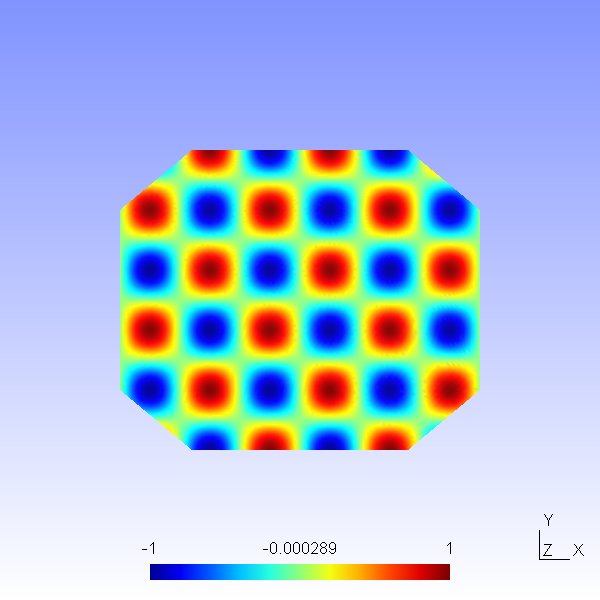
\includegraphics[width=6cm]{Figures/Helmholtz2D}
\caption{Solution of the 2D Helmholtz Problem.}
\end{center}
\end{figure}

By writing FldToTecplot or FldToVtk instead of FldToGmsh in the previous command, Tecplot or Paraview can be used to visualize the results.

\subsection{Advection dominated mass transport in a pipe}

The following example demonstrates the application of the ADRsolver for modelling advection dominated mass transport in a straight pipe. 
Such a transport regime is encountered frequently when modelling mass transport in arteries. This is because the diffusion 
coefficient of small blood borne molecules, for example oxygen or adenosine triphosphate, is very small $O(10^{-10})$.

\textbf{Background}

The governing equation for modelling mass transport is the unsteady advection diffusion equation:
\begin{equation}
\dfrac{\partial u}{\partial t}  + v\nabla u +  \epsilon \nabla^2 u = 0
\end{equation}

For small diffusion coefficient, $\epsilon$, the transport is dominated by advection and this leads to a very fine boundary
 layer adjacent to the surface which must be captured in order to get a realistic representation of the wall mass transfer processes.
 This creates problems not only from a meshing perspective, but also numerically where classical oscillations 
 are observed in the solution due to under-resolution of the boundary layer.\\

The Graetz-Nusselt solution is an analytical solution of a developing mass (or heat) transfer boundary layer in a pipe. 
Previously this solution has been used as a benchmark for the accuracy of numerical methods to capture the fine 
boundary layer which develops for high Peclet number transport (the ratio of advection to diffusion). 
The solution is derived based on the assumption that the velocity field within the mass transfer boundary layer 
is linear i.e. the Schmidt number (the relative thickness of the momentum to mass transfer boundary layer) is sufficiently large. 
The analytical solution for the non-dimensional mass transfer at the wall is given by:
\begin{equation}
S h(z) = \dfrac{2^{4/3}(Pe R/z)^{1/3}}{g^{1/3}\Gamma(4/3)} , 
\end{equation}
where $z$ is the streamwise coordinate, $R$ the pipe radius, $\Gamma(4/3)$ an incomplete 
Gamma function and $Pe$ the Peclet number given by:
\begin{equation}
Pe = \dfrac{2 U R}{\epsilon}
\end{equation}

In the following we will numerically solver mass transport in a pipe and compare the calculated mass transfer 
at the wall with the Graetz-Nusselt solution. The Peclet number of the transport regime under consideration is 
750000, which is physiologically relevant.

\textbf{Geometry}

The geometry under consideration is a pipe of radius, $R = 0.5$ and length $l = 0.5$

\begin{figure}[h!]
\begin{center}
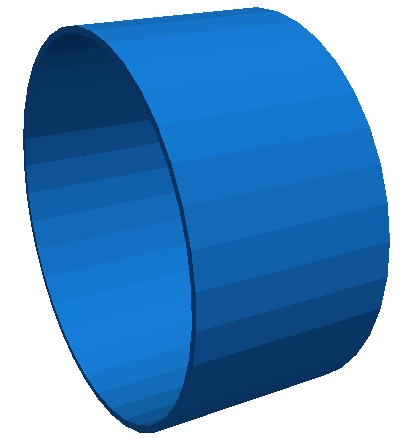
\includegraphics[width=6cm]{Figures/pipe}
\caption{Pipe.}
\end{center}
\end{figure}

Since the mass transport boundary layer will be confined to a very small layer adjacent to the wall we do not need to mesh
 the interior region, hence the mesh consists of a layer of ten prismatic elements over a thickness of 0.036R. 
The elements progressively grow over the thickness of domain.

\textbf{Input parameters}

\textbf{\footnotesize{Expansion}}

In this example we utilise heterogeneous polynomial order, in which the polynomial order normal to the wall is
 higher so that we avoid unphysical oscillations, and hence the incorrect solution, in the mass transport boundary layer.
  To do this we specify explicitly the expansion type, points type and distribution in each direction as follows:

\begin{lstlisting}[style=XMLStyle]
<EXPANSIONS>
  <E COMPOSITE="C[0]"
     NUMMODES="3,5,3"
     BASISTYPE="Modified_A,Modified_A,Modified_B"
     NUMPOINTS="4,6,3"
     POINTSTYPE="GaussLobattoLegendre,GaussLobattoLegendre,GaussRadauMAlpha1Beta0"
     FIELDS="u" />
</EXPANSIONS>
\end{lstlisting}

The above represents a quadratic polynomial order in the azimuthal and streamwise direction and 
4th order polynomial normal to the wall for a prismatic element.

\textbf{\footnotesize{Solver information}}

\begin{lstlisting}[style=XMLStyle]
<SOLVERINFO>
   <I PROPERTY="EQTYPE"                VALUE="UnsteadyAdvectionDiffusion" />
   <I PROPERTY="Projection"            VALUE="Continuous" />
   <I PROPERTY="DiffusionAdvancement"  VALUE="Implicit" />
   <I PROPERTY="AdvectionAdvancement"  VALUE="Explicit" />
   <I PROPERTY="TimeIntegrationMethod" VALUE="IMEXOrder1" />
   <I PROPERTY="GlobalSysSoln"         VALUE="IterativeStaticCond" />
</SOLVERINFO>
\end{lstlisting}

\textbf{\footnotesize{Parameters}}

\begin{lstlisting}[style=XMLStyle]
<PARAMETERS>
  <P> TimeStep = 0.0005              </P>
  <P> FinalTime = 30                 </P>
  <P> NumSteps = FinalTime/TimeStep  </P>
  <P> IO_CheckSteps = 1000           </P>
  <P> IO_InfoSteps = 200             </P>
  <P> epsilon = 1.33333e-6           </P>
</PARAMETERS>
\end{lstlisting}

The value of $\epsilon$ is $\epsilon = 1/Pe$.

\textbf{\footnotesize{Boundary conditions}}

The analytical solution represents a developing mass transfer boundary layer in a pipe. In order to 
reproduce this numerically we assume that the inlet concentration is a uniform value and the outer 
wall concentration is zero; this will lead to the development of the mass transport boundary layer along the length 
of the pipe. Since we do not model explicitly the mass transfer in the interior region of the pipe we assume that 
the inner wall surface concentration is the same as the inlet concentration; this assumption is valid based on the large 
Peclet number meaning the concentration boundary layer is confined to the region in the immediate vicinity of the wall.
 The boundary conditions are specified as follows in the input file:

\begin{lstlisting}[style=XMLStyle]
<BOUNDARYREGIONS>
   <B ID="0"> C[3] </B>  <!-- inlet -->
   <B ID="1"> C[4] </B>  <!-- outlet -->
   <B ID="2"> C[2] </B>  <!-- outer surface -->
   <B ID="3"> C[5] </B>  <!-- inner surface -->
</BOUNDARYREGIONS>

<BOUNDARYCONDITIONS>
  <REGION REF="0">
    <D VAR="u" VALUE="1" />
  </REGION>
  <REGION REF="1">
    <N VAR="u" VALUE="0" />
  </REGION>
  <REGION REF="2">
    <D VAR="u" VALUE="0" />
  </REGION>
  <REGION REF="3">
    <D VAR="u" VALUE="1" />
  </REGION>
</BOUNDARYCONDITIONS>
\end{lstlisting}


\textbf{\footnotesize{Functions}}

The velocity field within the domain is fully developed pipe flow (Poiseuille flow), hence we 
can define this through an analytical function as follows:

\begin{lstlisting}[style=XMLStyle]
<FUNCTION NAME="AdvectionVelocity">
  <E VAR="Vx" VALUE="0" />
  <E VAR="Vy" VALUE="0" />
  <E VAR="Vz" VALUE="2.0*(1-(x*x+y*y)/0.25)" />
</FUNCTION>
\end{lstlisting}

We assume that the initial domain concentration is uniform everywhere and the same as the inlet. This is defined by,

\begin{lstlisting}[style=XMLStyle]
<FUNCTION NAME="InitialConditions">
  <E VAR="u" VALUE="1" />
</FUNCTION>
\end{lstlisting}

\textbf{Results}

To compare with the analytical expression we numerically calculate the concentration gradient at the surface of the pipe. 
This is then plotted against the analytical solution by extracting the solution along a line in the streamwise direction.

\begin{figure}[h!]
\begin{center}
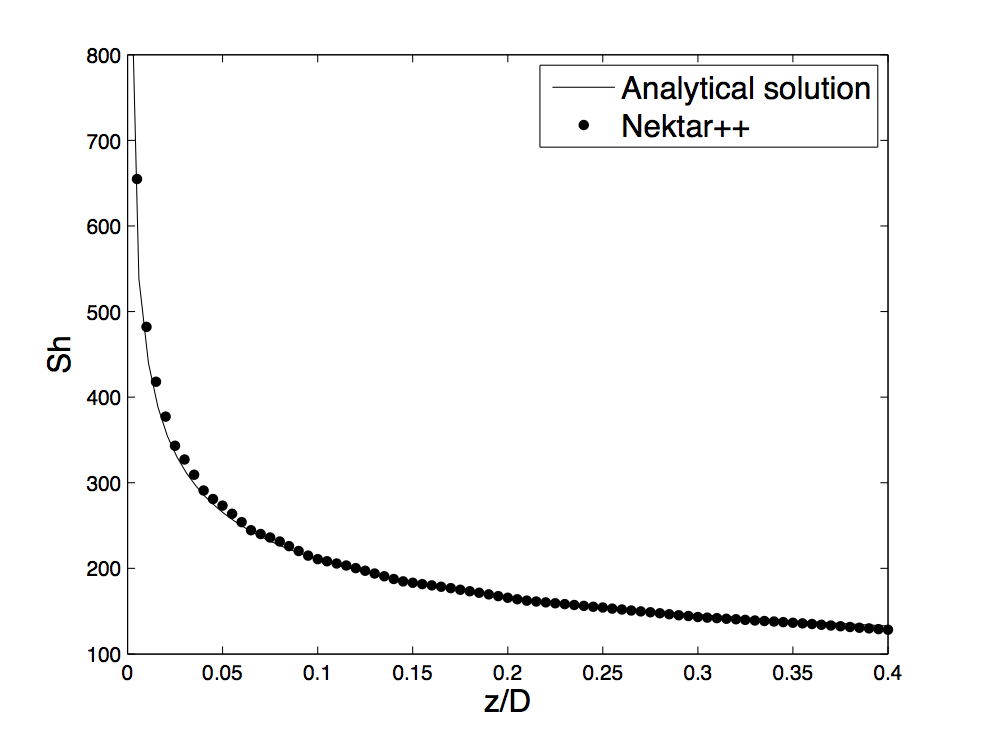
\includegraphics[width=7cm]{Figures/graetz-nusselt}
\caption{Concentration gradient at the surface of the pipe.}
\end{center}
\end{figure}



